
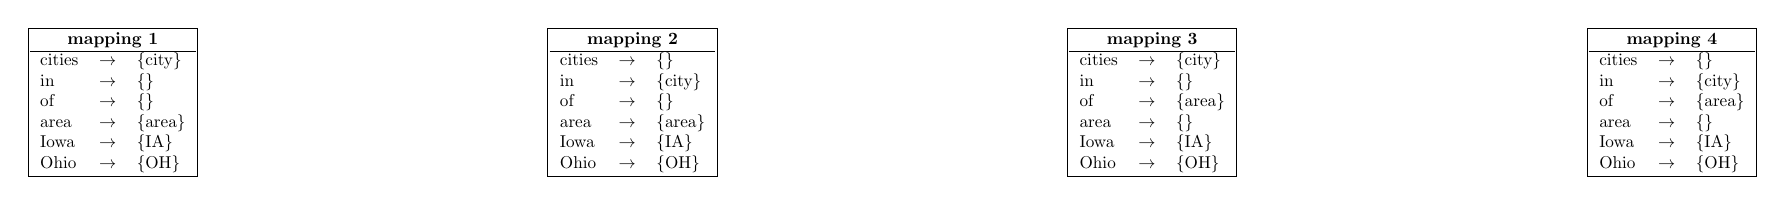
\begin{tikzpicture}
\tikzset{
    myarrow/.style={->, >=latex', shorten >=2pt},
	mybox/.style={
	scale=\scale,
%	rounded corners=.1em, 
	draw=black,
	inner sep=1,
%	text width=3cm,
},
}
\def\x{6.6}
\def\y{2.5}
\def\btw{5}
\def\scale{0.62}

	\node (A)[mybox] at (0,\y){
		\begin{tabular}{lll}
		\multicolumn{3}{c}{\bf mapping 1} \\ \hline
		 \nl{cities}&$\rightarrow$&\{\wl{city}\} \\
		 \nl{in}&$\rightarrow$&\{\} \\
		 \nl{of}&$\rightarrow$  &\{\} \\
		 \nl{area}&$\rightarrow$ & \{\wl{area}\} \\
		 \nl{Iowa}&$\rightarrow$ & \{\wl{IA}\} \\
		\nl{Ohio}&$\rightarrow$ & \{\wl{OH}\} \\
		\end{tabular}
	};

	
	\node (B) [mybox]at (\x,\y){
			\begin{tabular}{lll}
		\multicolumn{3}{c}{\bf mapping 2} \\ \hline
		 \nl{cities}&$\rightarrow$&\{\wl{}\} \\
	 \nl{in}&$\rightarrow$&\{\wl{city}\} \\
		 \nl{of}&$\rightarrow$  &\{\} \\
		 \nl{area}&$\rightarrow$ & \{\wl{area}\} \\
		 \nl{Iowa}&$\rightarrow$ & \{\wl{IA}\} \\
		\nl{Ohio}&$\rightarrow$ & \{\wl{OH}\} \\
		\end{tabular}
	};

	
	\node (C) [mybox]at (2*\x ,\y){
			\begin{tabular}{lll}
		\multicolumn{3}{c}{\bf mapping 3} \\ \hline
		 \nl{cities}&$\rightarrow$&\{\wl{city}\} \\
	 \nl{in}&$\rightarrow$&\{\} \\
		 \nl{of}&$\rightarrow$  &\{\wl{area}\} \\
		 \nl{area}&$\rightarrow$ & \{\wl{}\} \\
		 \nl{Iowa}&$\rightarrow$ & \{\wl{IA}\} \\
		\nl{Ohio}&$\rightarrow$ & \{\wl{OH}\} \\
		\end{tabular}
	};


	\node (D) [mybox]at (3*\x ,\y){
		\begin{tabular}{lll}
		\multicolumn{3}{c}{\bf mapping 4} \\ \hline
		 \nl{cities}&$\rightarrow$&\{\wl{}\} \\
	 \nl{in}&$\rightarrow$&\{\wl{city}\} \\
		 \nl{of}&$\rightarrow$  &\{\wl{area}\} \\
		 \nl{area}&$\rightarrow$ & \{\wl{}\} \\
		 \nl{Iowa}&$\rightarrow$ & \{\wl{IA}\} \\
		\nl{Ohio}&$\rightarrow$ & \{\wl{OH}\} \\
		\end{tabular}
	};
      

\end{tikzpicture}

